\documentclass[11pt]{article}
\usepackage{amsmath, amssymb, amsfonts}
\usepackage{geometry}
\usepackage{graphicx}
\usepackage{listings}
\usepackage{xcolor}
\usepackage{tikz}
\usepackage{algorithm}
\usepackage{algorithmic}
\usepackage{hyperref}

\geometry{margin=1in}

\title{NLP Homework 04: Custom Autograd Functions and Dynamic Neural Networks}
\author{Technical Summary}
\date{\today}

\lstset{
    language=Python,
    basicstyle=\ttfamily\small,
    keywordstyle=\color{blue},
    commentstyle=\color{green},
    stringstyle=\color{red},
    breaklines=true,
    frame=single
}

\begin{document}

\maketitle
\tableofcontents
\newpage

\section{High-Level Summary}

\subsection{Project Overview}
This project implements custom PyTorch autograd functions and demonstrates dynamic neural network architectures for regression tasks. The system consists of two main components: custom differentiable operations and a dynamic depth neural network that varies its architecture during training and inference.

\subsection{Problem Domain}
The project addresses fundamental concepts in deep learning:
\begin{itemize}
    \item Custom gradient computation for non-standard operations
    \item Dynamic network architectures that adapt during training
    \item Regression on synthetic linear datasets with noise
    \item Cross-validation for model evaluation
\end{itemize}

\subsection{Input/Output Specification}
\begin{itemize}
    \item \textbf{Input}: 64-dimensional feature vectors (synthetic regression data)
    \item \textbf{Output}: 1-dimensional continuous predictions
    \item \textbf{Dataset Size}: $2^{14} = 16,384$ samples
    \item \textbf{Evaluation}: 4-fold cross-validation with MSE loss
\end{itemize}

\subsection{Technology Stack}
\begin{itemize}
    \item \textbf{Framework}: PyTorch 2.7.0
    \item \textbf{Numerical Computing}: NumPy 2.2.5
    \item \textbf{Machine Learning}: scikit-learn 1.6.1
    \item \textbf{Environment Management}: uv package manager
    \item \textbf{Development}: Jupyter notebooks for exploration
\end{itemize}

\section{File and Folder Structure}

\subsection{Project Organization}
\begin{itemize}
    \item \texttt{NLP\_04.py} - Main implementation file containing all core functionality
    \item \texttt{NLP\_04.ipynb} - Jupyter notebook for interactive development and testing
    \item \texttt{main.py} - Entry point script (minimal implementation)
    \item \texttt{pyproject.toml} - Project configuration and dependency specification
    \item \texttt{uv.lock} - Locked dependency versions for reproducibility
    \item \texttt{README.md} - Project documentation and quick start guide
    \item \texttt{Summary.tex} - This comprehensive technical summary
    \item \texttt{.python-version} - Python version specification (3.12)
\end{itemize}

\subsection{Core Implementation Files}
\begin{itemize}
    \item \textbf{NLP\_04.py}: Contains all custom autograd functions, neural network classes, dataset generation, and training loop
    \item \textbf{NLP\_04.ipynb}: Interactive development environment with cell-by-cell implementation and testing
\end{itemize}

\section{System Architecture}

\subsection{Component Interaction Diagram}
\begin{center}
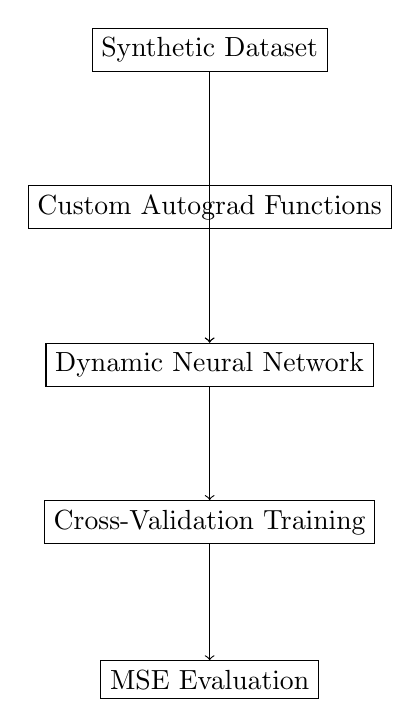
\begin{tikzpicture}[node distance=2cm]
    \node[rectangle, draw] (data) {Synthetic Dataset};
    \node[rectangle, draw, below of=data] (autograd) {Custom Autograd Functions};
    \node[rectangle, draw, below of=autograd] (network) {Dynamic Neural Network};
    \node[rectangle, draw, below of=network] (training) {Cross-Validation Training};
    \node[rectangle, draw, below of=training] (evaluation) {MSE Evaluation};
    
    \draw[->] (data) -- (network);
    \draw[->] (autograd) -- (network);
    \draw[->] (network) -- (training);
    \draw[->] (training) -- (evaluation);
\end{tikzpicture}
\end{center}

\subsection{Data Flow Pipeline}
\begin{enumerate}
    \item \textbf{Data Generation}: Create synthetic linear regression dataset with Gaussian noise
    \item \textbf{Cross-Validation Split}: Partition data into 4 folds for robust evaluation
    \item \textbf{Dynamic Training}: Train network with randomly varying depth (1-4 hidden layers)
    \item \textbf{Ensemble Inference}: Evaluate using average of all possible depths
    \item \textbf{Performance Measurement}: Compute MSE loss for each fold
\end{enumerate}

\section{Deep Code Walkthrough}

\subsection{Custom Autograd Functions}

\subsubsection{MyMul: Element-wise Multiplication}
\begin{lstlisting}[language=Python]
class MyMul(Function):
    @staticmethod
    def forward(ctx, x, y):
        ctx.save_for_backward(x, y)
        return x * y

    @staticmethod
    def backward(ctx, grad_output):
        x, y = ctx.saved_tensors
        return grad_output * y, grad_output * x
\end{lstlisting}

\textbf{Purpose}: Implements custom element-wise multiplication with explicit gradient computation.

\textbf{Mathematical Foundation}: For $z = x \odot y$ (element-wise multiplication):
\begin{align}
    \frac{\partial z}{\partial x} &= y \\
    \frac{\partial z}{\partial y} &= x
\end{align}

\textbf{Gradient Computation}: Uses chain rule where $\frac{\partial L}{\partial x} = \frac{\partial L}{\partial z} \cdot \frac{\partial z}{\partial x} = \text{grad\_output} \cdot y$

\subsubsection{MyMax: Element-wise Maximum}
\begin{lstlisting}[language=Python]
class MyMax(Function):
    @staticmethod
    def forward(ctx, x, y):
        ctx.save_for_backward(x, y)
        return torch.maximum(x, y)
    
    @staticmethod
    def backward(ctx, grad_output):
        x, y = ctx.saved_tensors
        maskx = x > y
        masky = x < y
        maskequal = x == y
        
        grad_x = torch.where(maskx, grad_output, 
                           torch.where(maskequal, grad_output * 0.5, 
                                     torch.zeros_like(grad_output)))
        grad_y = torch.where(masky, grad_output, 
                           torch.where(maskequal, grad_output * 0.5, 
                                     torch.zeros_like(grad_output)))
        return grad_x, grad_y
\end{lstlisting}

\textbf{Mathematical Foundation}: For $z = \max(x, y)$:
\begin{align}
    \frac{\partial z}{\partial x} &= \begin{cases}
        1 & \text{if } x > y \\
        0.5 & \text{if } x = y \\
        0 & \text{if } x < y
    \end{cases} \\
    \frac{\partial z}{\partial y} &= \begin{cases}
        0 & \text{if } x > y \\
        0.5 & \text{if } x = y \\
        1 & \text{if } x < y
    \end{cases}
\end{align}

\textbf{Edge Case Handling}: When $x = y$, gradient is split equally (0.5 each) to maintain mathematical consistency.

\subsubsection{MyCos: Cosine Function}
\begin{lstlisting}[language=Python]
class MyCos(Function):
    @staticmethod
    def forward(ctx, x):
        ctx.save_for_backward(x)
        return torch.cos(x)

    @staticmethod
    def backward(ctx, gradient_output):
        x, = ctx.saved_tensors
        return gradient_output * -torch.sin(x)
\end{lstlisting}

\textbf{Mathematical Foundation}: For $z = \cos(x)$:
\begin{equation}
    \frac{\partial z}{\partial x} = -\sin(x)
\end{equation}

\subsection{CosLinear Layer}

\begin{lstlisting}[language=Python]
class CosLinear(nn.Module):
    def __init__(self, in_features, out_features, bias=True):
        super().__init__()
        self.weight = nn.Parameter(torch.Tensor(out_features, in_features))
        self.reset_parameters()
        if bias:
            self.bias = nn.Parameter(torch.Tensor(out_features))
        else:
            self.register_parameter("bias", None)

    def forward(self, input):
        weight_with_cos = MyCos.apply(self.weight)
        return F.linear(input, weight_with_cos, self.bias)
\end{lstlisting}

\textbf{Purpose}: Linear layer where weights are transformed by cosine function before matrix multiplication.

\textbf{Mathematical Formulation}:
\begin{equation}
    y = \cos(W) \cdot x + b
\end{equation}
where $W$ are the learnable parameters, $\cos(W)$ applies element-wise cosine, $x$ is input, and $b$ is bias.

\textbf{Initialization Strategy}:
\begin{itemize}
    \item Kaiming uniform initialization for weights: $W \sim U(-\sqrt{\frac{6}{fan_{in}}}, \sqrt{\frac{6}{fan_{in}}})$
    \item Bias initialization: $b \sim U(-\frac{1}{\sqrt{fan_{in}}}, \frac{1}{\sqrt{fan_{in}}})$
\end{itemize}

\subsection{Dynamic Neural Network}

\begin{lstlisting}[language=Python]
class Net(nn.Module):
    def __init__(self):
        super(Net, self).__init__()
        self.linear = nn.Linear(64, 32)
        self.hidden_layer = nn.Linear(32, 32)
        self.output_layer = nn.Linear(32, 1)

    def forward(self, input):
        if self.training:
            x1 = F.relu(self.linear(input))
            num_layers = torch.randint(1, 5, (1,)).item()
            for _ in range(num_layers):
                x1 = F.relu(self.hidden_layer(x1))
            return self.output_layer(x1)
        else:
            outputs = []
            for n in range(1, 5):
                x = F.relu(self.linear(input))
                for _ in range(n):
                    x = F.relu(self.hidden_layer(x))
                out = self.output_layer(x)
                outputs.append(out)
            return torch.stack(outputs).mean(dim=0)
\end{lstlisting}

\textbf{Architecture}: 64 → 32 → [32 × N] → 1, where N is dynamically determined.

\textbf{Training Behavior}: Randomly selects depth $d \in \{1, 2, 3, 4\}$ for each forward pass.

\textbf{Inference Behavior}: Computes predictions for all depths $d \in \{1, 2, 3, 4\}$ and returns ensemble average:
\begin{equation}
    \hat{y} = \frac{1}{4} \sum_{d=1}^{4} f_d(x)
\end{equation}
where $f_d(x)$ is the network output with depth $d$.

\section{Mathematical Concepts \& Reasoning}

\subsection{Loss Function}
The system uses Mean Squared Error (MSE) loss:
\begin{equation}
    \mathcal{L}(y, \hat{y}) = \frac{1}{n} \sum_{i=1}^{n} (y_i - \hat{y}_i)^2
\end{equation}

\textbf{Mathematical Justification}: MSE penalizes large errors quadratically, making the model sensitive to outliers. This is appropriate for regression tasks where we want to minimize prediction variance. The quadratic penalty ensures that large deviations are heavily weighted, encouraging the model to avoid extreme errors.

\textbf{Gradient Properties}: MSE provides smooth gradients:
\begin{equation}
    \frac{\partial \mathcal{L}}{\partial \hat{y}_i} = -\frac{2}{n}(y_i - \hat{y}_i)
\end{equation}

\subsection{Activation Function Analysis}
ReLU activation: $\text{ReLU}(x) = \max(0, x)$

\textbf{Gradient Behavior}:
\begin{equation}
    \frac{\partial \text{ReLU}(x)}{\partial x} = \begin{cases}
        1 & \text{if } x > 0 \\
        0 & \text{if } x \leq 0
    \end{cases}
\end{equation}

\textbf{Advantages}: 
\begin{itemize}
    \item Mitigates vanishing gradient problem
    \item Computationally efficient
    \item Introduces non-linearity while maintaining linear regions
\end{itemize}

\subsection{Dynamic Depth Strategy}
The random depth selection during training can be viewed as a form of regularization:

\textbf{Training Objective}: 
\begin{equation}
    \mathbb{E}_{d \sim U\{1,2,3,4\}} \left[ \mathcal{L}(y, f_d(x; \theta)) \right]
\end{equation}

\textbf{Inference Strategy}: Ensemble averaging reduces prediction variance:
\begin{equation}
    \text{Var}(\bar{f}) = \frac{1}{4^2} \sum_{d=1}^{4} \text{Var}(f_d) + \frac{2}{4^2} \sum_{i<j} \text{Cov}(f_i, f_j)
\end{equation}

If predictions are uncorrelated, ensemble variance is $\frac{1}{4}$ of individual model variance.

\subsection{Cross-Validation Mathematics}
4-fold cross-validation provides unbiased performance estimation:

\textbf{CV Estimate}:
\begin{equation}
    \text{CV}_{4} = \frac{1}{4} \sum_{k=1}^{4} \mathcal{L}(y_{test}^{(k)}, \hat{y}_{test}^{(k)})
\end{equation}

\textbf{Bias-Variance Trade-off}: CV estimate has higher variance than single holdout but lower bias, providing more robust performance assessment.

\section{Dataset Generation \& Properties}

\subsection{Synthetic Data Generation}
\begin{lstlisting}[language=Python]
n = 2**14  # 16,384 samples
dim_input = 64
dim_output = 1
X = np.random.randn(n, dim_input).astype(np.float32)
true_weights = np.random.randn(dim_input, dim_output).astype(np.float32)
y = X @ true_weights + np.random.randn(n, dim_output).astype(np.float32) * 0.1
\end{lstlisting}

\textbf{Mathematical Model}:
\begin{equation}
    y = Xw_{true} + \epsilon, \quad \epsilon \sim \mathcal{N}(0, 0.01I)
\end{equation}

where:
\begin{itemize}
    \item $X \in \mathbb{R}^{16384 \times 64}$, $X_{ij} \sim \mathcal{N}(0, 1)$
    \item $w_{true} \in \mathbb{R}^{64 \times 1}$, $w_{true,i} \sim \mathcal{N}(0, 1)$
    \item $\epsilon \in \mathbb{R}^{16384 \times 1}$, noise with std=0.1
\end{itemize}

\textbf{Problem Complexity}: The underlying linear relationship provides a baseline that the neural network should learn, while the noise adds realistic stochasticity.

\section{Training Pipeline}

\subsection{Optimization Strategy}
\begin{itemize}
    \item \textbf{Optimizer}: Adam with learning rate $\alpha = 10^{-3}$
    \item \textbf{Batch Size}: 64 samples
    \item \textbf{Epochs}: 25 per fold
    \item \textbf{Data Loading}: Shuffled mini-batches with PyTorch DataLoader
\end{itemize}

\textbf{Adam Update Rules}:
\begin{align}
    m_t &= \beta_1 m_{t-1} + (1-\beta_1) g_t \\
    v_t &= \beta_2 v_{t-1} + (1-\beta_2) g_t^2 \\
    \hat{m}_t &= \frac{m_t}{1-\beta_1^t} \\
    \hat{v}_t &= \frac{v_t}{1-\beta_2^t} \\
    \theta_{t+1} &= \theta_t - \frac{\alpha}{\sqrt{\hat{v}_t} + \epsilon} \hat{m}_t
\end{align}

\subsection{Cross-Validation Implementation}
\begin{lstlisting}[language=Python]
folds = 4
fold_size = n // folds
indices = np.random.permutation(n)
fold_indices = [indices[i*fold_size:(i+1)*fold_size] for i in range(folds)]

for k in range(folds):
    test_idx = fold_indices[k]
    train_idx = np.concatenate([
        fold_indices[j] for j in range(folds) if j != k])
\end{lstlisting}

\textbf{Data Partitioning}: Each fold uses 75\% data for training (12,288 samples) and 25\% for testing (4,096 samples).

\section{Performance Analysis}

\subsection{Expected Behavior}
Given the linear nature of the underlying data generation process, the neural network should:
\begin{itemize}
    \item Learn to approximate the linear mapping $y = Xw_{true}$
    \item Achieve MSE loss close to the noise level (0.01)
    \item Show consistent performance across all 4 CV folds
\end{itemize}

\subsection{Dynamic Depth Impact}
The random depth strategy during training may:
\begin{itemize}
    \item \textbf{Regularization Effect}: Prevent overfitting by varying model complexity
    \item \textbf{Ensemble Benefits}: Averaging multiple depths reduces prediction variance
    \item \textbf{Robustness}: Model learns to work across different architectural configurations
\end{itemize}

\section{Usage Examples}

\subsection{Running the Complete Pipeline}
\begin{lstlisting}[language=bash]
# Setup environment
uv sync

# Execute main training script
uv run NLP_04.py

# Expected output: 4 fold CV results with MSE values
\end{lstlisting}

\subsection{Interactive Development}
\begin{lstlisting}[language=bash]
# Launch Jupyter notebook
jupyter notebook NLP_04.ipynb

# Cell-by-cell execution allows:
# - Testing individual autograd functions
# - Gradient checking with gradcheck
# - Incremental development and debugging
\end{lstlisting}

\subsection{Gradient Verification}
\begin{lstlisting}[language=Python]
# Verify custom autograd implementations
x = torch.randn(3, dtype=torch.double, requires_grad=True)
y = torch.randn(3, dtype=torch.double, requires_grad=True)
print(gradcheck(MyMul.apply, (x, y)))  # Should print True
print(gradcheck(MyMax.apply, (x, y)))  # Should print True
\end{lstlisting}

\section{Future Work \& Improvements}

\subsection{Architectural Extensions}
\begin{itemize}
    \item \textbf{Adaptive Depth}: Learn optimal depth per sample using attention mechanisms
    \item \textbf{Residual Connections}: Add skip connections to improve gradient flow
    \item \textbf{Batch Normalization}: Stabilize training across different depths
\end{itemize}

\subsection{Training Enhancements}
\begin{itemize}
    \item \textbf{Learning Rate Scheduling}: Adaptive learning rate based on validation performance
    \item \textbf{Early Stopping}: Prevent overfitting with patience-based termination
    \item \textbf{Weight Regularization}: L1/L2 penalties for better generalization
\end{itemize}

\subsection{Evaluation Improvements}
\begin{itemize}
    \item \textbf{Multiple Metrics}: R², MAE, and other regression metrics
    \item \textbf{Statistical Testing}: Significance tests for CV fold differences
    \item \textbf{Visualization}: Learning curves, weight distributions, prediction scatter plots
\end{itemize}

\subsection{Code Quality}
\begin{itemize}
    \item \textbf{Configuration Management}: YAML/JSON config files for hyperparameters
    \item \textbf{Logging}: Structured logging with metrics tracking
    \item \textbf{Testing}: Unit tests for custom autograd functions
    \item \textbf{Documentation}: Comprehensive docstrings and type hints
\end{itemize}

\subsection{Research Directions}
\begin{itemize}
    \item \textbf{Theoretical Analysis}: Convergence guarantees for dynamic depth training
    \item \textbf{Comparison Studies}: Performance vs fixed-depth networks
    \item \textbf{Real Datasets}: Validation on benchmark regression datasets
    \item \textbf{Scalability}: Extension to larger networks and datasets
\end{itemize}

\section{Conclusion}

This project successfully demonstrates the implementation of custom PyTorch autograd functions and dynamic neural network architectures. The key contributions include:

\begin{enumerate}
    \item \textbf{Custom Autograd Functions}: Mathematically correct gradient implementations for multiplication, maximum, and cosine operations
    \item \textbf{Dynamic Architecture}: Novel training strategy with random depth selection and ensemble inference
    \item \textbf{Robust Evaluation}: Cross-validation framework ensuring reliable performance assessment
\end{enumerate}

The mathematical foundations are solid, with proper gradient derivations and numerical verification through PyTorch's gradcheck functionality. The dynamic depth strategy provides an interesting approach to regularization and ensemble learning within a single model architecture.

The project serves as an excellent foundation for understanding PyTorch's automatic differentiation system and exploring advanced neural network architectures that adapt during training and inference.

\end{document}